\chapter{Analysis of Variance}

The main idea of an ANOVA test is that if researchers ask if a set of sample means gives 
evidence of differences in the population means, what matters is not how far apart 
the sample means are, but how far apart they are \textit{relative to the variability of 
individual observations}.

\section{One-way ANOVA}

\begin{figure}[h!]
\centering
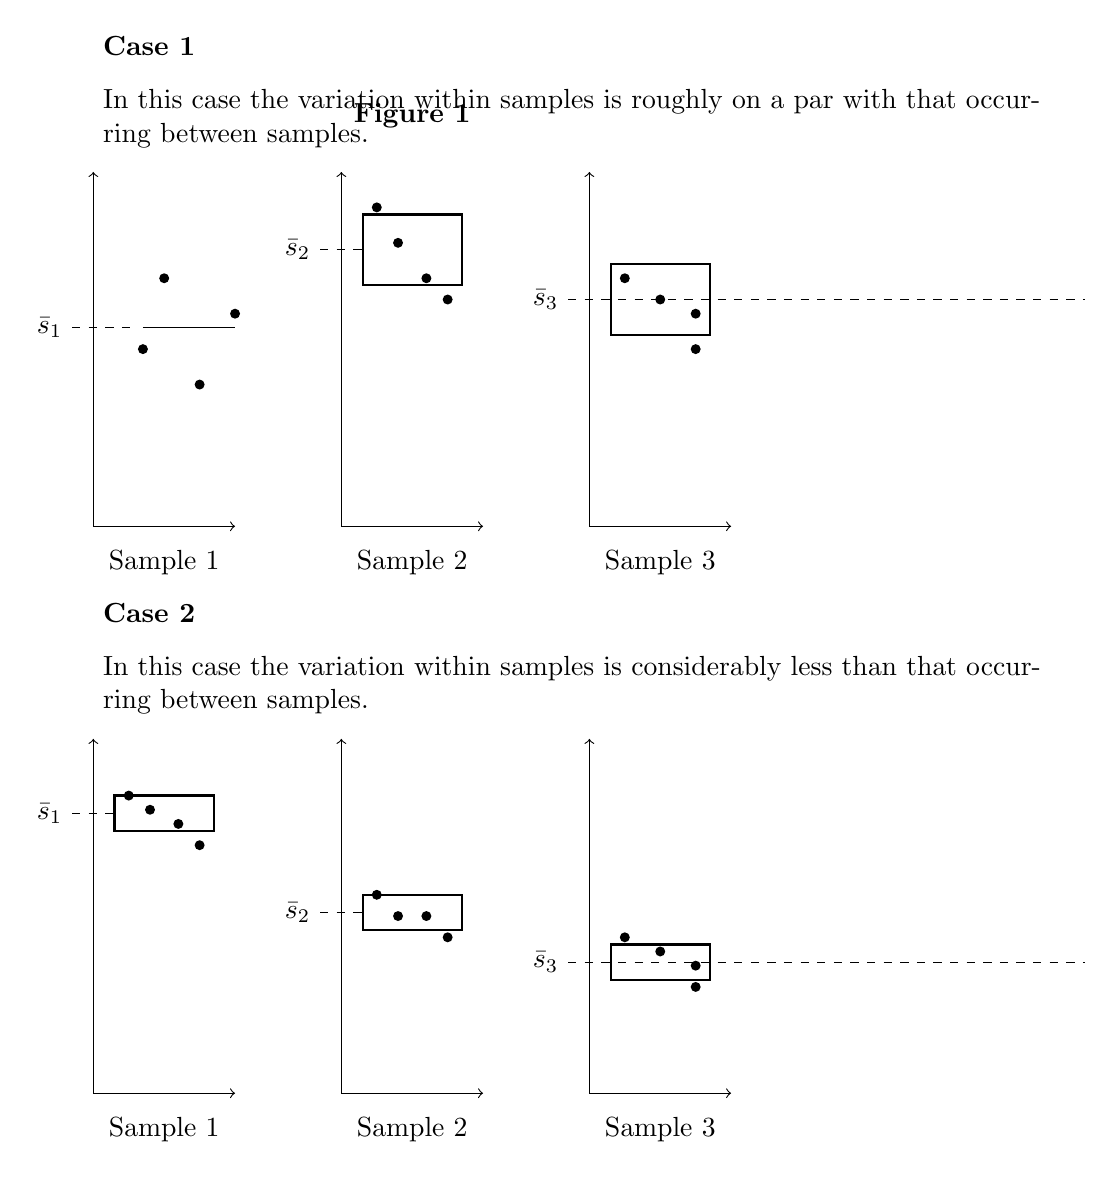
\begin{tikzpicture}[scale=0.9]
% Case 1
    \node[anchor=south west] at (0,6.5) {\textbf{Case 1}};
    \node[anchor=north west, text width=12cm] at (0,6.3) {In this case the variation within samples is roughly on a par with that occurring between samples.};

    % Sample 1 - Case 1
    \begin{scope}[shift={(0,0)}]
        \draw[->] (0,0) -- (0,5) node[midway,left] {};
        \draw[->] (0,0) -- (2,0);
        \node[below] at (1,-0.2) {Sample 1};
        % Data points
        \fill (0.7,2.5) circle (2pt);
        \fill (1,3.5) circle (2pt);
        \fill (1.5,2.0) circle (2pt);
        \fill (2,3.0) circle (2pt);
        % Box showing mean
        %\draw[thick] (0.3,2.3) rectangle (1.7,3.3);
        % Mean line
        \draw[dashed] (-0.3,2.8) -- (0.6,2.8);
        \draw[solid] (0.7,2.8) -- (2,2.8);
        \node[left] at (-0.3,2.8) {$\bar{s}_1$};
    \end{scope}

    % Sample 2 - Case 1
    \begin{scope}[shift={(3.5,0)}]
        \draw[->] (0,0) -- (0,5);
        \draw[->] (0,0) -- (2,0);
        \node[below] at (1,-0.2) {Sample 2};
        % Data points
        \fill (0.5,4.5) circle (2pt);
        \fill (0.8,4.0) circle (2pt);
        \fill (1.2,3.5) circle (2pt);
        \fill (1.5,3.2) circle (2pt);
        % Box showing mean
        \draw[thick] (0.3,3.4) rectangle (1.7,4.4);
        % Mean line
        \draw[dashed] (-0.3,3.9) -- (0.3,3.9);
        \node[left] at (-0.3,3.9) {$\bar{s}_2$};
    \end{scope}

    % Sample 3 - Case 1
    \begin{scope}[shift={(7,0)}]
        \draw[->] (0,0) -- (0,5);
        \draw[->] (0,0) -- (2,0);
        \node[below] at (1,-0.2) {Sample 3};
        % Data points
        \fill (0.5,3.5) circle (2pt);
        \fill (1.0,3.2) circle (2pt);
        \fill (1.5,3.0) circle (2pt);
        \fill (1.5,2.5) circle (2pt);
        % Box showing mean
        \draw[thick] (0.3,2.7) rectangle (1.7,3.7);
        % Mean line
        \draw[dashed] (-0.3,3.2) -- (7.0,3.2);
        \node[left] at (-0.3,3.2) {$\bar{s}_3$};
    \end{scope}

    \node at (4.5,5.8) {\textbf{Figure 1}};

    % Case 2
    \node[anchor=south west] at (0,-1.5) {\textbf{Case 2}};
    \node[anchor=north west, text width=12cm] at (0,-1.7) {In this case the variation within samples is considerably less than that occurring between samples.};

    % Sample 1 - Case 2
    \begin{scope}[shift={(0,-8)}]
        \draw[->] (0,0) -- (0,5);
        \draw[->] (0,0) -- (2,0);
        \node[below] at (1,-0.2) {Sample 1};
        % Data points (less variation)
        \fill (0.5,4.2) circle (2pt);
        \fill (0.8,4.0) circle (2pt);
        \fill (1.2,3.8) circle (2pt);
        \fill (1.5,3.5) circle (2pt);
        % Box showing mean
        \draw[thick] (0.3,3.7) rectangle (1.7,4.2);
        % Mean line
        \draw[dashed] (-0.3,3.95) -- (0.3,3.95);
        \node[left] at (-0.3,3.95) {$\bar{s}_1$};
    \end{scope}

    % Sample 2 - Case 2
    \begin{scope}[shift={(3.5,-8)}]
        \draw[->] (0,0) -- (0,5);
        \draw[->] (0,0) -- (2,0);
        \node[below] at (1,-0.2) {Sample 2};
        % Data points (less variation)
        \fill (0.5,2.8) circle (2pt);
        \fill (0.8,2.5) circle (2pt);
        \fill (1.2,2.5) circle (2pt);
        \fill (1.5,2.2) circle (2pt);
        % Box showing mean
        \draw[thick] (0.3,2.3) rectangle (1.7,2.8);
        % Mean line
        \draw[dashed] (-0.3,2.55) -- (0.3,2.55);
        \node[left] at (-0.3,2.55) {$\bar{s}_2$};
    \end{scope}

    % Sample 3 - Case 2
    \begin{scope}[shift={(7,-8)}]
        \draw[->] (0,0) -- (0,5);
        \draw[->] (0,0) -- (2,0);
        \node[below] at (1,-0.2) {Sample 3};
        % Data points (less variation)
        \fill (0.5,2.2) circle (2pt);
        \fill (1.0,2.0) circle (2pt);
        \fill (1.5,1.8) circle (2pt);
        \fill (1.5,1.5) circle (2pt);
        % Box showing mean
        \draw[thick] (0.3,1.6) rectangle (1.7,2.1);
        % Mean line
        \draw[dashed] (-0.3,1.85) -- (7.0,1.85);
        \node[left] at (-0.3,1.85) {$\bar{s}_3$};
    \end{scope}
\end{tikzpicture}
\caption{Comparison of within-sample and between-sample variation in ANOVA}
\label{fig:anova_samples}
\end{figure}

\begin{lemma}
    \label{lem:an01}
    The total sum of squares is equal to the \textit{sum of within} and \textit{between sum of squares}, that is 
    \begin{equation}
        \CS{T} = \CS{W} + \CS{B}.
    \end{equation}
\end{lemma}
\begin{proof}
    Rewriting we have 
    \begin{align*}
        \CS{T} &= \sum^m_{i=1} \sum^n_{j=1} (Y_{ij} - \ols{Y}_{\bullet \bullet })\\
        &= \sum^m_{i=1} \sum^n_{j=1} \left[ (Y_{ij} - \ols{Y}_{i \bullet }) + (Y_{i\bullet} - \ols{Y}_{\bullet \bullet }) \right]^2\\
        &= \sum^m_{i=1} \sum^n_{j=1} (Y_{ij} - \ols{Y}_{i \bullet })^2 + \sum^m_{i=1} \sum^n_{j=1}(Y_{i\bullet} - \ols{Y}_{\bullet \bullet })^2
        + 2 \sum^m_{i=1} \sum^n_{j=1} (Y_{ij} - \ols{Y}_{i \bullet })(Y_{i\bullet} - \ols{Y}_{\bullet \bullet })\\
    \end{align*}
    Hence we obtain the asserted result
    \[
        \CS{T} = \CS{W} + \CS{B}
    \]
    and the proof of the lemma is complete.
\end{proof}

\begin{theorem}
    Suppose the one-way ANOVA model is given by the equation 
    where the $\varepsilon_{ij}$'s are independent and normally 
    distributed random variables with mean zero and variance 
    $\sigma^2$ for $i = 1,2,\ldots, m$ and $j = 1,2,\ldots,n$.
    
    The null hypothesis 
    \[
        H_0 : \mu_1 = \mu_2 = \cdots = \mu_m = \mu
    \]
    is rejected whenever the statistics $\mathcal{F}$ satisfies 
    \begin{equation}
        \mathcal{F} = \frac{\CS{B} / (m-1)}{\CS{W} / [m(n-1)]} > F_\alpha(m-1, m(n-1)).
    \end{equation}

    where $\alpha$ is the significance level of the hypothesis test and $F_\alpha(m-1, m(n-1))$ 
    denotes the $100(1 - \alpha)$-th percentile of the $F$-distribution with $m-1$ numerator 
    and $m(n-1)$ denominator degrees of freedom.
\end{theorem}
\begin{proof}
    Under the null hypothesis $H_0 : \mu_1 = \mu_2 = \cdots = \mu_m = \mu$, the likelihood function 
    takes the form 
    \begin{align*}
        L(\mu, \sigma^2 | Y) &= \prod^m_{i=1} \prod^n_{j=1} \left\{ \frac{1}{\sqrt{2\sigma^2}}
        \exp \left[ - \frac{(Y_{ij} - \mu)^2 }{2\sigma^2}\right] \right\}\\
        &= \left( \frac{1}{ \sqrt{2\sigma^2}} \right)^{nm} \exp \left[ - \frac{1}{2\sigma^2} \sum^{m}_{i=1} \sum^n_{j=1} (Y_{ij} - \mu)^2\right]
        \label{eq:an1.0} \tag{{\color{red} $\heartsuit $}}
    \end{align*}
    Maximizing the natural logarithm of the likelihood function \eqref{eq:an1.0}, we obtain 
    \[
        \widehat{\mu} = \ols{Y}_{\bullet \bullet} \quad \text{ and }
        \quad 
        \widehat{\sigma_{H_0}} = \frac{1}{mn} \CS{T}
    \]
    as the maximum likelihood estimators of $\mu$ and $\sigma^2$, respectively. Plugging these 
    estimators back into \eqref{eq:an1.0}, we have the maximum likelihood function, that is,
    \[
        \max L(\mu, \sigma^2 | Y) = \left( \frac{1}{ \sqrt{2\widehat{\sigma^2_{H_0}}}} \right)^{nm} \exp \left[ - \frac{1}{2\widehat{\sigma^2_{H_0}}} \sum^{m}_{i=1} \sum^n_{j=1} (Y_{ij} - \ols{Y}_{\bullet \bullet})^2\right].
    \]
    Simplifying the above expression, we see that 
    \begin{align*}
        \max L(\mu, \sigma^2 | Y) &= \left( \frac{1}{ \sqrt{2\widehat{\sigma^2_{H_0}}}} \right)^{nm} \exp \left[ - \left(\frac{2}{nm} \CS{T} \right)^{-1} \sum^{m}_{i=1} \sum^n_{j=1} (Y_{ij} - \ols{Y}_{\bullet \bullet})^2\right]\\
        &= \left( \frac{1}{ \sqrt{2\widehat{\sigma^2_{H_0}}}} \right)^{nm} \exp \left[ - \frac{nm}{2 \, \CS{T}} \CS{T} \right]\\
        &=  \left( \frac{1}{ \sqrt{2\widehat{\sigma^2_{H_0}}}} \right)^{nm} e^{-\mfrac{nm}{2}}  \label{eq:an1.1} \tag{{\color{cyan} $\clubsuit $}}
    \end{align*}

    When no restrictions imposed, we obtain the maximum of the likelihood function from\\ \cref{lem:an01} as
    \[
        \max L(\mu_1, \mu_2, \ldots, \mu_m, \sigma^2 | Y)
        = \left( \frac{1}{ \sqrt{2\widehat{\sigma^2_{H_0}}}} \right)^{nm} \exp \left[ - \frac{1}{2\widehat{\sigma^2_{H_0}}} \sum^{m}_{i=1} \sum^n_{j=1} (Y_{ij} - {\color{red} \ols{Y}_{i \bullet}})^2\right]
        \label{eq:an1.2} \tag{{\color{orange!50!white} $\bigstar $}}
    \]
    notice that the grand mean $\ols{Y}_{\bullet \bullet}$ now replace by $\ols{Y}_{i \bullet}$, 
    and $\widehat{\sigma^2_{H_0}}$ being replace by $\widehat{\sigma^2}$. Again 
    simplying the expression above and 
    \begin{align*}
        \max L(\mu_1, \mu_2, \ldots, \mu_m, \sigma^2 | Y) &= \left( \frac{1}{ \sqrt{2\widehat{\sigma^2}}} \right)^{nm} \exp \left[ - \left(\frac{2}{nm} \CS{W} \right)^{-1} \sum^{m}_{i=1} \sum^n_{j=1} (Y_{ij} - \ols{Y}_{i \bullet})^2\right]\\
        &= \left( \frac{1}{ \sqrt{2\widehat{\sigma^2}}} \right)^{nm} \exp \left[ - \frac{nm}{2 \, \CS{W}} \CS{W} \right]\\
        &=  \left( \frac{1}{ \sqrt{2\widehat{\sigma^2}}} \right)^{nm} e^{-\mfrac{nm}{2}}.
    \end{align*}

    Next, we are going to find the likelihood ratio statistic $\Lambda$ for testing the null hypothesis $H_0$. 
    Recall that the likelihood ratio statistic $\Lambda$ can be found by evaluating 
    \[
        \Lambda = \frac{\max L(\mu, \sigma^2)}{\max L(\mu_1, \mu_2, \ldots, \mu_m, \sigma^2)}.
    \]
    Using \eqref{eq:an1.1} divide \eqref{eq:an1.2}, we have 
    \[
        \Lambda = \left( \frac{\widehat{\sigma^2} }{\widehat{\sigma^2_{H_0}}} \right)^{\mfrac{nm}{2}}.
    \]
    Recall that the likelihood ratio test to reject the null hypothesis is 
    \[
        \Lambda < k_0 \implies \left( \frac{\widehat{\sigma^2} }{\widehat{\sigma^2_{H_0}}} \right)^{\mfrac{nm}{2}} < k_0 
        \implies \frac{\widehat{\sigma^2_{H_0}}}{ \widehat{\sigma^2}} > \left( \frac{1}{k_0} \right)^{\mfrac{2}{nm}}
    \]
    Applying \cref{lem:an01},
    \[
        \frac{\CS{W} + \CS{B}}{\CS{W}} > \left( \frac{1}{k_0} \right)^{\mfrac{2}{nm}} \implies 
        \frac{\CS{B}}{\CS{W}} > k' \label{eq:an1.3} \tag{{\color{gray} $\spadesuit $}}
    \]
    where $\displaystyle k' := \left( \frac{1}{k_0} \right)^{\mfrac{2}{nm}} - 1$. In order to find the 
    cutoff point $k'$ in \eqref{eq:an1.3}. We apply \cref{lem:an01}. Thus 
    \[
        \mathcal{F} = \frac{\CS{B} / (m-1)}{\CS{W} / (m(n-1))} > \frac{m(n-1)}{m-1}k'.
    \] 
\end{proof}

% Table fits to paper width using tabularx
\begin{table}[h!]
\renewcommand{\arraystretch}{1.2}
\begin{tabularx}{\textwidth}{cc c p{2.5cm} p{2.5cm}}
    \toprule
    Source of Variation & Sums of squares & Degree of freedom & Mean squares & $\mathcal{F}$-statistic \\[0.6em]
    \midrule
    Between & $\CS{B}$ & $m - 1$ & $\MS{B} = \mfrac{\CS{B}}{m-1}$ & $\displaystyle \mathcal{F} = \frac{\MS{B} }{\MS{W} }$ \\[0.6em]
    Within & $\CS{W}$ & $N - m$ & $\MS{W} = \mfrac{\CS{W}}{N-m}$ & \\
    \hline
    Total & $\CS{T}$ & $N - 1$ & & \\
    \bottomrule
\end{tabularx}
\caption{One-way ANOVA table with unequal sample size}
\end{table}

\section{Test for the Homogeneity of Variances}

One of the assumptions behind the ANOVA test is that the variances 
of each samples under consideration should be the same for all population.

The test statistic $B_c$ is given by
\begin{equation}
    B_c = \frac{(N -m) \ln S^2_p - \sum^m_{i=1} (n_i - 1) \ln s^2_i }{\displaystyle 1 + \frac{1}{3(m-1)} 
    \left[ \sum^m_{i=1} \frac{1}{n_i - 1} - \frac{1}{N - m} \right]}
\end{equation}
In the formula above, 
\begin{itemize}
    \item[$\bullet$] $s^2_i$ is the sample variance of the $i$-th group.
    \item[$\bullet$] $n_i$ is the sample size of $i$-th group.
    \item[$\bullet$] $N = \sum n_i$ is the total sample size.
    \item[$\bullet$] $m$ is the number of groups. 
\end{itemize}

and the pooled variance $S^2_p$ is given by
\begin{equation}
    S^2_p = \frac{\sum^m_{i=1} (n_i - 1) s^2_i}{N - m} = \MS{W}.
\end{equation}
The sampling distribution of $B_c$ is approximately chi-square with $m - 1$ degrees of freedom, that is,
\[
    B_c \sim \chi^2 (m-1)
\]
when $(n_i - 1) \geq 3$. Therefore the Barlett test rejects the null hypothesis 
$H_0 : \sigma^2_1 = \sigma^2_2 = \cdots = \sigma^2_m$ at a significance level $\alpha$ if 
\[
    B_c \sim \chi^2_{1 - \alpha} (m-1)
\]
where $\chi^2_{1 - \alpha} (m-1)$ denotes the upper $(1 - \alpha) \times 100$ percentile of the chi-square 
with $m-1$ degrees of freedom.

\begin{definition}[Barlett's test]
    The test statistic for Barlett's test is 
    \begin{equation}
        B_c = \frac{(N -m) \ln S^2_p - \sum^m_{i=1} (n_i - 1) \ln S^2_i }{\displaystyle 1 + \frac{1}{3(m-1)} 
    \left[ \sum^m_{i=1} \frac{1}{n_i - 1} - \frac{1}{N - m} \right]}.
    \end{equation}
    Reject $H_0 : \sigma^2_1 = \sigma^2_2 = \cdots = \sigma^2_m$ if $B_c > \chi^2_\alpha(m-1)$.
\end{definition}

Barlett's test is the uniformly most powerful (UMP) test for the homogeneity of variances 
problem under the assumption that each treatment population is normally distributed.
Bartlett's test is useful whenever the assumption of equal variances is made. In particular, this assumption is made for the frequently used one-way analysis of variance.

However, Barlett's test has crucial weaknesses if the normality assumption is not met:
\begin{itemize}
    \item[$\bullet$] The tests reliability is sensitive (not robust) to non-normality.
    \item[$\bullet$]  If the treatment populations are not approximately normal, the true significance level can be
 very different from the nominal significance level (say, $ \alpha = 0.05$). This difference depends on the
 kurtosis (4th moment) of the distribution.
\end{itemize}

 In this case, Bartlett's or Levene's test should be applied to verify the assumption.

\subsection{Levene's test}

 The Bartlett's test assumes that the grouped samples should be taken from
 normal populations. Thus Bartlett test is sensitive to departures from
 normality. The Levene's test is an alternative to the Bartlett's test that is less
 sensitive to departures from normality. Levene (1960) proposed a test for the
 homogeneity of population variances that considers the random variables

\begin{definition}[Levene's Test]
    To perform Levene's Test:
    \begin{enumerate}
        \item Calculate each $Z_{ij} = |Y_{ij} - \ols{Y}_{i \bullet}|$.
        \item Run an ANOVA on the set of $Z_{ij}$ values.
        \item If $\mathcal{F} > F_{\alpha}(m - 1, N-m)$, reject null hypothesis 
        $H_0 : \sigma^2_1 = \sigma^2_2 = \cdots = \sigma^2_m$ and conclude that 
        the variances are not all equal.
    \end{enumerate}
\end{definition}

 Brown and Forsythe (1974) proposed using the transformed variables based
 on the absolute deviations from the median,that is 
 \begin{equation}
    Z_{ij} = |Y_{ij} - \widetilde{Y}_{i \bullet}|,
 \end{equation}
 where $\widetilde{Y}_{i \bullet}$ denotes the median of $i$-th group. Again if the $F$-test is 
 significant, the homogeneity of variances is rejected.

\begin{definition}[Brown-Forsythe Test]
    To perform Brown-Forsythe's Test:
    \begin{enumerate}
        \item Calculate each $Z_{ij} = |Y_{ij} - \widetilde{Y}_{i \bullet}|$, 
            where $\widetilde{Y}_{i \bullet}$ is the $i$-th median of the treatment.
        \item Run an ANOVA on the set of $Z_{ij}$ values.
        \item If $\mathcal{F} > F_{\alpha}(m - 1, N-m)$, reject null hypothesis 
        $H_0 : \sigma^2_1 = \sigma^2_2 = \cdots = \sigma^2_m$ and conclude that 
        the variances are not all equal.
    \end{enumerate}
\end{definition}

\begin{example}
    For the following data set contains 10 measurements of gear diameter (in centimeter)
    for five different batches for a total of 50 measurements.

    \begin{table}[!htbp]
        \centering
        \begin{tabular}{ccccc}
            \toprule
            \multicolumn{5}{c}{Batches}\\[0.5em]
            1 & 2 & 3 & 4 & 5\\
            \midrule
            1.006 & 0.998 & 0.991 & 1.005 & 0.998\\
            0.996 & 1.006 & 0.987 & 1.002 & 0.998\\
            0.998 & 1.000 & 0.997 & 0.994 & 0.982\\
            1.000 & 1.002 & 0.999 & 1.000 & 0.990\\
            0.992 & 0.997 & 0.995 & 0.995 & 1.002\\
            0.993 & 0.998 & 0.994 & 0.994 & 0.984\\
            1.002 & 0.996 & 1.000 & 0.998 & 0.996\\
            0.999 & 1.000 & 0.999 & 0.996 & 0.993\\
            0.994 & 1.006 & 0.996 & 1.002 & 0.980\\
            1.000 & 0.988 & 0.996 & 0.996 & 1.018\\
            \bottomrule
        \end{tabular}
    \end{table}

\end{example}

The Cochran's $C$ test statistic is popular for test equivalence of variances among multiple sample groups.
It is a one-sided upper limit variance outlier test, and it is simple to apply with the following assumptions:
\begin{itemize}
    \item[$\bullet$] The data in each group are normally distributed.
    \item[$\bullet$] The data set is balanced design, i.e., each group has the same sample size.
\end{itemize}

The Cochran's $C$-test has been used as an alternative to Bartlett, Levene and Brown
Forsythe's tests in the evaluation of homoscedasticity (same 
variance) such as in a linear regression model. Note that  
this Cochran's C test is totally different with the Cochran's $Q$ test, which the last one is being used in the 
analysis of two-way randomized block designs with different treatments in a 
design of experiments.

\begin{equation}
    C = \frac{\displaystyle \max\limits_{1 \leq i \leq m} s^2_i}{\displaystyle \sum^m_{i=1} s^2_i}.
\end{equation}

The test statistic is the ratio of the maximum variance among the data set, and the sum of 
all the variances. 

\section*{Tutorials}

\begin{mdframed}
    \vspace{-0.25cm}
    \hspace{-0.25cm}
    \begin{Exercise}
        Given 20 observations on breakdown voltage for some materials
        \begin{center}
            \begin{tabular}{cccccccccc}
            24.46 & 25.61 & 26.25 & 26.42 & 26.66 & 27.15 & 27.31 & 27.54 & 27.74 & 27.94\\
            27.98 & 28.04 & 28.28 & 28.49 & 28.50 & 28.87 & 29.11 & 29.13 & 29.50 & 30.88\\
            \end{tabular}
        \end{center}
    \end{Exercise}
\end{mdframed}


